% Human Digital Twin — Detailed Project Report
\documentclass[12pt,a4paper]{article}

\usepackage[utf8]{inputenc}
\usepackage{amsmath,amssymb,amsfonts}
\usepackage{graphicx}
\usepackage[hidelinks,pageanchor=false]{hyperref}
\usepackage{bookmark}
\usepackage{geometry}
\usepackage{titlesec}
\usepackage{enumitem}
\usepackage{fancyhdr}
\usepackage{lastpage}
\usepackage{xcolor}
\usepackage{float}
\usepackage{booktabs}
\usepackage{longtable}
\usepackage{array}
\usepackage{multirow}
\usepackage{tikz}
\usetikzlibrary{shapes,arrows.meta,positioning,fit,backgrounds}
\usepackage{listings}
\usepackage{parskip}
\setlength{\parskip}{6pt plus 1pt}
\setlength{\headheight}{14pt}

\geometry{top=1in, bottom=1in, left=1in, right=1in}
\graphicspath{{Images/}}
\newcommand{\img}[2][]{\includegraphics[#1]{\detokenize{#2}}}

% ── Page style ──────────────────────────────────────────────────────────────
\pagestyle{fancy}
\fancyhf{}
\fancyhead[L]{\small\textcolor{headingblue}{\textit{Human Digital Twin — Project Report}}}
\fancyhead[R]{\small\textcolor{headingblue}{VIT Vellore}}
\fancyfoot[C]{\thepage}
\renewcommand{\headrulewidth}{0.4pt}

% ── Colours & headings ──────────────────────────────────────────────────────
\definecolor{headingblue}{RGB}{0,51,160}
\definecolor{codegreen}{rgb}{0,0.55,0}
\definecolor{codegray}{rgb}{0.5,0.5,0.5}
\definecolor{codepurple}{rgb}{0.45,0,0.7}
\definecolor{backcolour}{rgb}{0.96,0.96,0.94}

\titleformat{\section}
  {\normalfont\Large\bfseries\color{headingblue}}{\thesection}{1em}{}
\titleformat{\subsection}
  {\normalfont\large\bfseries}{\thesubsection}{1em}{}

% ── Code listing style ───────────────────────────────────────────────────────
\lstdefinestyle{mystyle}{
    backgroundcolor=\color{backcolour},
    commentstyle=\color{codegreen},
    keywordstyle=\color{magenta},
    numberstyle=\tiny\color{codegray},
    stringstyle=\color{codepurple},
    basicstyle=\ttfamily\footnotesize,
    breakatwhitespace=false, breaklines=true,
    captionpos=b, keepspaces=true,
    numbers=left, numbersep=5pt,
    showspaces=false, showstringspaces=false,
    showtabs=false, tabsize=2
}
\lstset{style=mystyle}

% ── Title ────────────────────────────────────────────────────────────────────
\begin{document}

\begin{titlepage}
\centering
\vspace*{0.5cm}

{\Large\bfseries\color{headingblue}
  Vellore Institute of Technology, Vellore\\[4pt]}
{\large SENSE School (School of Electronics Engineering)\\[4pt]}
{\large Bachelor of Technology in Biomedical Engineering\\[0.8cm]}

\rule{\linewidth}{1.5pt}\\[0.4cm]
{\Huge\bfseries\color{headingblue} Human Digital Twin}\\[0.3cm]
{\Large\bfseries\color{headingblue}
  A Real-Time Clinical Dashboard \&\\
  AI-Powered Predictive Monitoring Platform}\\[0.3cm]
\rule{\linewidth}{1.5pt}\\[0.5cm]

{\large\textbf{Detailed Project Report}}\\[1.2cm]

\begin{tabular}{ll}
  \textbf{PRATIK KUMAR}             & \textcolor{headingblue}{\textbf{24BML0027}} \\[4pt]
  \textbf{UDAY KRISHAN KHANDELWAL} & \textcolor{headingblue}{\textbf{24BML0017}} \\[4pt]
  \textbf{THAKUR CHAND CHOUDHARY}  & \textcolor{headingblue}{\textbf{24BML0012}} \\[4pt]
  \textbf{SHRUTI}                  & \textcolor{headingblue}{\textbf{24BML0033}} \\[4pt]
  \textbf{VIDHI AGARWAL}           & \textcolor{headingblue}{\textbf{24BML0081}} \\
\end{tabular}

\vfill
\img[width=0.50\textwidth]{VIT_COLOURED LOGO.png}\\[0.6cm]
{\small Academic Year 2025--26}
\end{titlepage}

\thispagestyle{empty}
\tableofcontents
\newpage
\setcounter{page}{1}

% ============================================================================
\section{Field / Area of the Project}
% ============================================================================

This project resides at the intersection of \textbf{Health Informatics, Biomedical Engineering,
and Applied Artificial Intelligence}. Concretely, it encompasses the design and
implementation of an end-to-end \textit{Human Digital Twin} (HDT) framework tailored
for Intensive Care Unit (ICU) and general hospital telemetry. The platform deals with
continuous, multi-modal patient data ingestion, real-time physiological parameter
monitoring, automated laboratory-document parsing via Optical Character Recognition
(OCR), forward-looking risk prediction via Machine Learning (ML), clinical order
management (medications, laboratory tests, surgical schedules), and bed-occupancy
administration. By bridging edge-sensing microcontrollers with a cloud-style FastAPI
backend and a responsive React/TypeScript frontend, the project fundamentally targets
the operational digitisation of critical care environments in resource-constrained
settings such as government hospitals and medical colleges across India.

% ============================================================================
\section{Existing Work \& Publications}
% ============================================================================

Traditional ICU telemetry setups have historically relied on monolithic, proprietary
hardware platforms that trap patient data in siloed stores, making longitudinal
predictive analytics difficult. The following survey contextualises our contribution
within current research directions.

\textbf{MIMIC Datasets.}  The MIMIC-III \cite{johnson2016} and MIMIC-IV \cite{johnson2023} ecosystems established reproducible baselines for machine learning on electronic health records (EHR). Landmark models for mortality prediction, sepsis onset \cite{reyna2020}, and readmission risk emerged from these corpora \cite{celi2020}. However, deploying retrospective models in a live bedside interface without bespoke middleware remained an open engineering challenge—one that this project addresses directly.

\textbf{Human Digital Twins in Healthcare.}  El~Saddik \cite{elsaddik2018} introduced the concept of a digital twin converging multimedia signals into a persistent computational replica. Subsequent clinical interpretations \cite{bjornsson2019} highlight the potential for personalised treatment simulation, while noting that standardised real-time interfaces connecting hardware streams to the twin model are scarce. Rajpurkar \textit{et al.} \cite{rajpurkar2022} and Topol \cite{topol2019} further argue that AI will fundamentally reshape diagnostic and monitoring workflows.

\textbf{OCR in Clinical Settings.}  Microsoft's TrOCR \cite{trocr2021} and similar transformer-based OCR engines have demonstrated high accuracy on structured documents. However, their integration as a native module within a live patient dashboard—extracting lab values directly into a time-series database—is an underexplored contribution that our system realises. The EasyOCR library used here builds on the broader deep-learning-based OCR ecosystem validated in \cite{trocr2021}.

\textbf{Clinical-Grade ECG and Arrhythmia Detection.}  Hannun \textit{et al.} \cite{hannun2019} demonstrated cardiologist-level arrhythmia detection with CNNs on single-lead ECGs, while Kiranyaz \textit{et al.} \cite{kiranyaz2016} showed that patient-specific 1-D CNNs outperform generic models. The foundational ECG databases were established by Moody and Mark \cite{moody1999} and Goldberger \textit{et al.} \cite{goldberger2000}. The QRS detection algorithm by Pan and Tompkins \cite{pan1985} remains a preprocessing cornerstone. These findings motivate our AI prediction module which adapts dynamically to per-patient longitudinal data.

% ============================================================================
\section{Summary and Background of the Work}
% ============================================================================

Critical care environments impose substantial cognitive load on clinicians. Doctors
and nurses are simultaneously confronted with disparate data streams: bedside monitors
display real-time waveforms, EHR applications lock historical records behind
login-intensive workflows, and paper-based laboratory reports accumulate in physical
folders awaiting manual transcription. This fragmentation leads to delayed recognition
of deterioration events, medication errors, and a loss of longitudinal patient context
during shift handovers.

This project addresses the fragmentation by designing a unified \textbf{Human Digital
Twin} application from the ground up. The system centralises patient monitoring via a
full-stack platform: a Python/FastAPI backend and a React/TypeScript frontend operating
together on a local network, accessible on both desktop workstations and mobile devices
carried by physicians during ward rounds.

The platform operates as a \textbf{Master Patient Index (MPI)} that establishes unique
patient identities; a \textbf{Bed Board} that tracks physical hospital occupancy and
assigns patients to wards; a \textbf{Clinical Dashboard} that renders real-time
telemetry, continuous predictive risk scores, medication management, and order workflows;
and an \textbf{AI Module} that delivers heart failure risk forecasts and medication
recommendations grounded in the patient's active longitudinal twin data.  Furthermore,
to bridge the analog-to-digital gap present in the Indian clinical context, an OCR
pipeline can digest scanned paper lab reports and instantaneously ingest the extracted
values into the patient's twin timeline.

% ============================================================================
\section{Objectives}
% ============================================================================

\begin{enumerate}[label=\textbf{\arabic*.}, leftmargin=*, itemsep=4pt]
  \item \textbf{Centralise Patient Identity} — Build a robust Master Patient Index
        and encounter system capable of securely tracking large clinical cohorts with
        Indian demographic profiles.
  \item \textbf{Real-Time Telemetry and Dashboards} — Provide immediate visualisation
        of ECG traces, SpO$_2$, blood pressure, heart rate, and core vitals, updated
        dynamically as new readings arrive.
  \item \textbf{AI-Powered Predictive Decisions} — Implement predictive mortality and
        risk-trajectory modelling powered by the patient's real-time vitals and
        historical comorbidities, with automated medication recommendations for heart
        failure management.
  \item \textbf{Comprehensive Order Management} — Support clinical order workflows
        including medication orders, laboratory tests, order-set pathways, and result
        routing so the digital twin reflects all active clinical decisions.
  \item \textbf{Bed and Resource Administration} — Provide a Bed Board view enabling
        nurses and admission staff to manage unit occupancy and surgical/clinical
        schedules in real time.
  \item \textbf{Paper-to-Digital Automation} — Build an OCR pipeline that automatically
        parses physical lab reports (PDFs / images) into structured longitudinal databases,
        eliminating manual transcription.
  \item \textbf{Clinician Mobility} — Ensure the solution is fully responsive and
        accessible over a LAN so physicians can evaluate dashboards on mobile devices
        during rounds without a fixed workstation.
\end{enumerate}

% ============================================================================
\section{Working Principle}
% ============================================================================

The platform operates on a modernised \textit{three-tier web architecture} tightly
integrated with \textit{AI micro-services}.

\textbf{Ingestion Layer (Analog to Digital).}  Clinical variables enter the platform
through structured encounter forms completed at admission, direct REST API calls that
simulate or relay bedside device streams, and through the OCR pipeline that reads
scanned laboratory documents. The ingestion layer is stateless and idempotent—repeated
posts of the same observation simply record duplicate timestamps rather than corrupting
the patient record.

\textbf{Service \& Database Layer (Platform Backend).}  A FastAPI server handles HTTP
requests, validates schemas with Pydantic, and routes data to one of two SQLite
databases. The \texttt{hospital\_core} database manages administrative logic: the
Master Patient Index, active encounters, bed occupancy, physician orders, medication
records, laboratory results routing, and surgical/clinical schedules. The
\texttt{clinical\_patients} database is a purpose-built \textit{Digital Twin} store
handling high-frequency chronological time-series: vital-sign arrays, lab-value
timelines, and comorbidity states. This dual-database design separates transactional
consistency (administrative) from append-optimised time-series workloads (telemetry),
giving each layer the schema best suited to its access pattern.

\textbf{AI \& OCR Module.}  A separate endpoint layer hosts the predictive heart failure
risk model, which consumes features from the active digital twin (BNP, ejection fraction,
creatinine, HbA1c, comorbidity flags) and returns a probability score alongside
evidence-based medication recommendations. The OCR module wraps EasyOCR with a
domain-specific heuristic parser that anchors on standard clinical terminology to extract
structured lab values from free-form document images.

\textbf{Presentation Layer (Frontend User Interface).}  A React-based Single Page
Application (SPA) fetches and subscribes to patient state via REST.  Modular components—
\texttt{BedBoard}, \texttt{PatientSelect}, \texttt{ClinicalBoard}, \texttt{OrdersBoard},
and \texttt{NewEncounter}—render rich, interactive data visualisations including animated
charts, risk gauges, and Kanban-style order panels.

% ============================================================================
\section{Block Diagram}
% ============================================================================

\begin{figure}[H]
\centering
\setlength{\parskip}{0pt}%
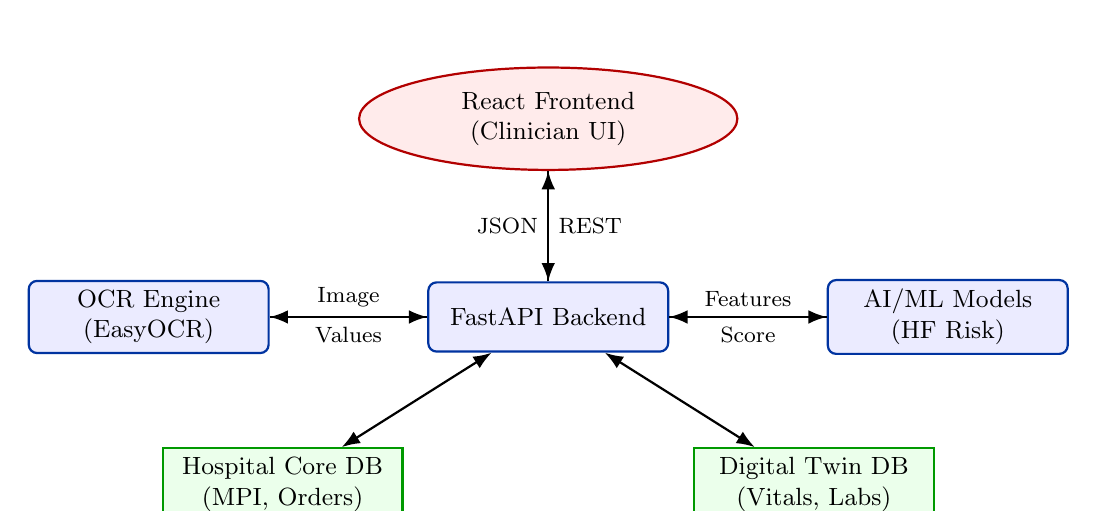
\begin{tikzpicture}[
  node distance=1.4cm and 2.0cm,
  >=Latex, thick,
  every node/.style={font=\small},
  block/.style={rectangle, draw=headingblue, fill=blue!8,
      text width=8em, align=center, rounded corners=3pt, minimum height=2.5em},
  db/.style={rectangle, draw=green!60!black, fill=green!8,
      text width=8em, align=center, minimum height=2.5em},
  ui/.style={ellipse, draw=red!70!black, fill=red!8,
      text width=9em, align=center, minimum height=2.5em}
]
\node[ui] (frontend) {React Frontend\\(Clinician UI)};
\node[block, below=of frontend] (api) {FastAPI Backend};
\node[block, left=of api]  (ocr) {OCR Engine\\(EasyOCR)};
\node[block, right=of api] (ml)  {AI/ML Models\\(HF Risk)};
\node[db, below left=1.2cm and 0.3cm of api]  (dbA) {Hospital Core DB\\(MPI, Orders)};
\node[db, below right=1.2cm and 0.3cm of api] (dbB) {Digital Twin DB\\(Vitals, Labs)};

\draw[->] (frontend) -- node[right,font=\footnotesize]{REST} (api);
\draw[->] (api) -- node[left,font=\footnotesize]{JSON} (frontend);
\draw[->] (api) -- node[above,font=\footnotesize]{Image} (ocr);
\draw[->] (ocr) -- node[below,font=\footnotesize]{Values} (api);
\draw[->] (api) -- node[above,font=\footnotesize]{Features} (ml);
\draw[->] (ml) -- node[below,font=\footnotesize]{Score} (api);
\draw[<->] (api) -- (dbA);
\draw[<->] (api) -- (dbB);
\end{tikzpicture}
\caption{System block diagram: React frontend interacts with FastAPI backend, which coordinates OCR/ML modules and dual SQLite databases.}
\label{fig:block}
\end{figure}

% ============================================================================
\section{Algorithm}
% ============================================================================

\subsection{Digital Twin Instantiation Algorithm}
\begin{enumerate}[label=\textbf{Step \arabic*.}, leftmargin=*, itemsep=3pt]
  \item \textbf{Input:} Patient demographic details, chief complaint, baseline vitals,
        ongoing medications, and comorbidity flags (diabetes, hypertension, smoking, etc.).
  \item \textbf{Identity Resolution.}  Check whether an \texttt{existingPatientId} is
        supplied. If yes, locate and update the existing MPI record. If no, generate a
        unique identifier (\texttt{PT-XXXX}) and Medical Record Number (\texttt{MRN-XXXXXXX}).
  \item \textbf{Encounter Initiation.}  Create a new encounter row in the
        \texttt{encounters} table (status: \textit{Admitted}), timestamped to the
        current ISO datetime.
  \item \textbf{Twin Structuring.}  Insert or update the patient row in
        \texttt{clinical\_patients.db} with serialised JSON blobs for demographics and
        comorbidities; mark \texttt{active\_status = `active'}.
  \item \textbf{Baseline Telemetry Ingestion.}  Commit the first vital-sign readings
        (HR, Systolic/Diastolic BP, SpO$_2$, RR) and laboratory values (EF, creatinine,
        sodium, potassium, BNP, HbA1c, cholesterol, haemoglobin) against the encounter
        timestamp into the time-series tables.
  \item \textbf{Medication Hydration.}  For each submitted medication, insert a row
        into \texttt{medication\_history} with dosage, timing, and source
        (\textit{Admission Intake}).
  \item \textbf{Isolated JSON Snapshot.}  Write a self-contained
        \texttt{PT-XXXX.json} file to \texttt{data/PatientDatabase/} for offline model
        inference and backup.
  \item \textbf{Output:}  Return \texttt{patient\_id}, \texttt{mrn}, success status.
        Frontend navigates to the active Clinical Dashboard for that patient.
\end{enumerate}

\subsection{OCR Laboratory Ingestion Algorithm}
\begin{enumerate}[label=\textbf{Step \arabic*.}, leftmargin=*, itemsep=3pt]
  \item \textbf{Input:}  Image or PDF byte-stream of a physical lab report.
  \item \textbf{OCR Processing.}  Extract raw text blocks using EasyOCR or
        LayoutLM; bounding boxes preserve spatial relationships between labels and values.
  \item \textbf{Semantic Anchoring.}  Iterate through text blocks searching for
        recognised medical anchors (``Haemoglobin'', ``HbA1c'', ``Sodium'', ``Creatinine'',
        ``Platelet Count'', etc.) from a controlled clinical vocabulary.
  \item \textbf{Value-Unit Correlation.}  Extract numeric values and SI units
        physically adjacent to each anchor; apply sanity ranges to discard artefacts.
  \item \textbf{Database Committal.}  \texttt{INSERT} each extracted lab into
        \texttt{lab\_values} mapped to the active \texttt{patient\_id} with the current
        timestamp.
  \item \textbf{Output:}  Updated patient timelines rendered immediately in the
        dashboard without any manual transcription.
\end{enumerate}

% ============================================================================
\section{Code}
% ============================================================================

\subsection{Backend — Digital Twin Encounter Endpoint (Python/FastAPI)}
\begin{lstlisting}[language=Python, caption=Core encounter creation route in \texttt{hospital\_core.py}]
@router.post("/encounter")
async def create_new_encounter(encounter: NewEncounterModel):
    """Hydrate a new Digital Twin from admission clinical parameters."""
    patient_id = (encounter.existingPatientId
                  if encounter.existingPatientId
                  else f"PT-{random.randint(2000, 9999):04d}")
    timestamp = datetime.now().isoformat()
    h_conn = get_db_connection()        # hospital_core.db
    c_conn = get_clinical_db_connection()  # clinical_patients.db
    try:
        # ---- 1. MPI upsert ------------------------------------------------
        mrn = f"MRN-{random.randint(1000000, 9999999)}"
        h_cursor.execute('''
            INSERT INTO patients
              (id, mrn, first_name, last_name, dob, gender, phone, address)
            VALUES (?, ?, ?, ?, ?, ?, ?, ?)
        ''', (patient_id, mrn, encounter.firstName, encounter.lastName,
              encounter.dob, encounter.gender,
              encounter.phone, encounter.address))

        # ---- 2. Encounter row ---------------------------------------------
        h_cursor.execute('''
            INSERT INTO encounters
              (visit_id, patient_id, unit, status, admission_time)
            VALUES (?, ?, 'CVICU', 'Admitted', ?)
        ''', (f"ENC-{random.randint(10000,99999)}", patient_id, timestamp))

        # ---- 3. Digital Twin time-series ----------------------------------
        c_cursor.execute('''
            INSERT INTO patients
              (patient_id, demographics, comorbidities, active_status)
            VALUES (?, ?, ?, 'active')
        ''', (patient_id, json.dumps(demographics), json.dumps(comorbidities)))

        for name, val, unit in vital_list:
            c_cursor.execute(
                "INSERT INTO vital_signs "
                "(patient_id, timestamp, vital_name, value, unit) "
                "VALUES (?, ?, ?, ?, ?)",
                (patient_id, timestamp, name, val, unit))

        h_conn.commit(); c_conn.commit()
        return {"patient_id": patient_id, "status": "success"}
    except Exception as e:
        h_conn.rollback(); c_conn.rollback()
        raise HTTPException(status_code=500, detail=str(e))
\end{lstlisting}

\subsection{Frontend — Patient Selection with Encounter Routing (TypeScript/React)}
\begin{lstlisting}[language=Java, caption=Patient table row with encounter navigation in \texttt{PatientSelect.tsx}]
const handleAddEncounter = (patient: Patient) => {
  navigate(`/new-encounter?patientId=${patient.id}`);
};
// Inside the table row render:
<button
  className="btn-encounter"
  onClick={() => handleAddEncounter(p)}
>
  ADD ENCOUNTER
</button>
\end{lstlisting}

% ============================================================================
\section{Results Snapshot}
% ============================================================================

The following screenshots document the complete clinical workflow of the platform,
sequenced from patient admission through medication management, AI risk assessment,
OCR lab ingestion, order management, bed administration, and scheduling.

% --- 1. New Encounter -------------------------------------------------------
\subsection{New Encounter — Digital Twin Initiation}
When a patient arrives at the hospital, the attending physician or admissions nurse
opens the \textit{New Encounter} form. All demographic fields, comorbidity checkboxes,
baseline vitals, and current medications are captured in a single scrollable form.
Upon submission, the system simultaneously creates an MPI record, an encounter entry,
and initialises the patient's Digital Twin in the time-series database.

\begin{figure}[H]
\centering
\img[width=0.90\textwidth]{New encounter dashboard.png}
\caption{New Encounter form — capturing demographics, vitals, comorbidities, and
  baseline medications to hydrate the Digital Twin at admission.}
\label{fig:newenc}
\end{figure}

% --- 2. Ongoing Medication ---------------------------------------------------
\subsection{Ongoing Medications at Admission}
Alongside the primary encounter data, the clinician enters the patient's ongoing
medication regimen including drug name, dosage (e.g., 5~mg, 2.5~mg), and timing
schedule (before breakfast, after lunch, etc.). These entries are stored in
\texttt{medication\_history} and rendered in the patient's active chart throughout
their hospital stay.

\begin{figure}[H]
\centering
\img[width=0.90\textwidth]{Ongoing mediction of new encounter.png}
\caption{Ongoing medication panel within the New Encounter workflow — drug, dosage,
  and timing details persisted directly to the Digital Twin's medication history.}
\label{fig:ongoingmed}
\end{figure}

% --- 3. Patient Clinical Dashboard (without AI) ------------------------------
\subsection{Clinical Dashboard — Real-Time Telemetry Overview}
Once the encounter is saved, the application navigates to the Clinical Board for that
specific patient. This view presents live vital-sign trends (HR, BP, SpO$_2$, RR) as
animated charts, the patient banner (name, MRN, age, code status), alert triggers, and
the active medication list — all without requiring any AI inference, allowing the
dashboard to load immediately with purely deterministic data.

\begin{figure}[H]
\centering
\img[width=0.92\textwidth]{pateint Dashboard without AI predection.png}
\caption{Clinical Board (pre-AI) — real-time telemetry panel showing vital-sign sparklines,
  patient banner, and active chart immediately after encounter creation.}
\label{fig:clinboard}
\end{figure}

% --- 4. AI Prediction Dashboard ---------------------------------------------
\subsection{AI Prediction — Heart Failure Risk Modelling}
Clicking the \textit{AI Prediction} tab loads the machine-learning inference panel.
The model — trained on MIMIC-IV-derived heart failure cohorts — ingests the patient's
current BNP, ejection fraction, creatinine, sodium, HbA1c, and comorbidity flags
to produce a holistic risk probability score alongside a personalised treatment
recommendation summary displayed in natural language.

\begin{figure}[H]
\centering
\img[width=0.92\textwidth]{Ai prediction dashboard.png}
\caption{AI Prediction Dashboard — heart failure risk probability gauge, feature
  importance breakdown, and model-generated medication recommendations.}
\label{fig:aipred}
\end{figure}

% --- 5. AI Prediction Graph -------------------------------------------------
\subsection{AI Prediction Graph and Recommended Medications}
To complement the summary gauge, the platform renders a detailed feature-contribution
graph and a ranked list of recommended medications with evidence-grading labels.
This output is derived from the same inference pass and gives the clinician a transparent
view of \textit{why} a particular risk score was assigned.

\begin{figure}[H]
\centering
\img[width=0.90\textwidth]{AI pred graph and recom mediction for HF.png}
\caption{AI prediction feature graph and evidence-based medication recommendations for
  heart failure management within the Digital Twin platform.}
\label{fig:aigraph}
\end{figure}

% --- 6. OCR Lab Ingestion ---------------------------------------------------
\subsection{OCR-Based Laboratory Report Ingestion}
Physical lab reports—printed by hospital pathology departments—can be uploaded
directly to the patient's record. The OCR pipeline extracts values such as haemoglobin,
platelet count, serum sodium, and creatinine from the scanned image and appends them to
the longitudinal twin database, eliminating manual re-entry and the errors associated
with it.

\begin{figure}[H]
\centering
\img[width=0.88\textwidth]{OCR extraction from report.png}
\caption{OCR lab-report ingestion — scanned document processed by EasyOCR; structured
  lab values (Hb, platelets, Na, creatinine) extracted and appended to the patient's
  digital twin timeline.}
\label{fig:ocr}
\end{figure}

% --- 7. MPI -----------------------------------------------------------------
\subsection{Master Patient Index}
The Master Patient Index (MPI) serves as the single source of truth for all patient
identities within the hospital. Clinicians can search by name, MRN, or patient ID
to locate existing records. The table displays demographic essentials and provides a
direct button to open the Clinical Dashboard or initiate a new encounter for that
patient.

\begin{figure}[H]
\centering
\img[width=0.92\textwidth]{MPI.png}
\caption{Master Patient Index — searchable registry of 1{,}000+ patients with Indian
  demographic profiles, providing one-click access to Clinical Boards and encounter
  creation.}
\label{fig:mpi}
\end{figure}

% --- 8. Medication Orders ---------------------------------------------------
\subsection{Orders Board — Medication Orders}
The Orders Board offers a dedicated panel for placing new medication orders within
an active encounter. The physician selects a drug from the autocomplete (sourced from
the India A–Z medicines dataset), specifies dosage, route, and frequency, and submits
the order. The record is immediately reflected in the patient's active chart.

\begin{figure}[H]
\centering
\img[width=0.92\textwidth]{Medication order.png}
\caption{Medication order panel — physician ordering interface with drug autocomplete,
  dosage, route selection, and real-time commit to the patient's Digital Twin record.}
\label{fig:medorder}
\end{figure}

% --- 9. Order Sets & Pathways -----------------------------------------------
\subsection{Order Sets and Clinical Pathways}
To accelerate common workflows, the platform provides pre-defined order sets and
clinical pathways (e.g., \textit{Acute Heart Failure Management}, \textit{Sepsis
Bundle}, \textit{Post-Cardiac Cath Care}). A clinician activates a pathway by
clicking one button, which instantiates all associated medication and laboratory orders
simultaneously, minimising the chance of omission.

\begin{figure}[H]
\centering
\img[width=0.92\textwidth]{order sets pathways.png}
\caption{Order sets and clinical pathways panel — one-click activation of evidence-based
  care bundles that simultaneously place all linked medication and laboratory orders.}
\label{fig:ordersets}
\end{figure}

% --- 10. Laboratory Orders --------------------------------------------------
\subsection{Orders Board — Laboratory Orders}
Separate from medication orders, the laboratory ordering panel allows physicians to
request specific investigations (CBC, LFT, RFT, cardiac enzymes, ABG, etc.) directly
from the dashboard. Orders are timestamped, linked to the encounter, and appear in the
Results Routing inbox once reported by the laboratory.

\begin{figure}[H]
\centering
\img[width=0.92\textwidth]{Laboratory order.png}
\caption{Laboratory order panel — investigation request interface allowing physicians to
  order CBCs, metabolic panels, and cardiac enzymes directly from the Digital Twin
  dashboard.}
\label{fig:laborder}
\end{figure}

% --- 11. Results Routing (Inbox) --------------------------------------------
\subsection{Results Routing — Clinical Inbox}
Completed laboratory results are routed to the ordering physician's inbox, prioritised
by clinical urgency. Critical values are highlighted in red, ``final'' results in blue,
and ``pending'' in amber. The clinician can view the result in context, acknowledge
it, and link it back to the patient's timeline with a single click.

\begin{figure}[H]
\centering
\img[width=0.92\textwidth]{Resluts routing.png}
\caption{Results routing inbox — provider-centric view of pending and final laboratory
  results, sorted by urgency with direct linking back to the ordering encounter.}
\label{fig:results}
\end{figure}

% --- 12. Bed Board ----------------------------------------------------------
\subsection{Bed Board / Unit View}
The Bed Board provides a real-time occupancy map of each hospital unit. Each card
represents one bed, displaying the current patient name, MRN, admission time, acuity
level, and attending physician. New admissions from the encounter flow appear
immediately at the top (most recent first), enabling charge nurses to manage
unit capacity efficiently.

\begin{figure}[H]
\centering
\img[width=0.92\textwidth]{Bed boards.png}
\caption{Bed Board / Unit View — real-time occupancy display sorted by most recent
  admission; new encounters from the Digital Twin flow appear immediately at the top.}
\label{fig:bedboard}
\end{figure}

% --- 13. Surgical and Clinical Schedule ------------------------------------
\subsection{Surgical and Clinical Schedule}
The scheduling module provides the attending physician with a consolidated view of
the day's surgical theatre bookings and outpatient clinic slots. Procedures are
organised chronologically with patient name, procedure type, estimated duration,
and theatre assignment, allowing the clinical team to anticipate workload transitions
between the ICU and theatre.

\begin{figure}[H]
\centering
\img[width=0.92\textwidth]{Surgical and clinical schedule.png}
\caption{Surgical and clinical schedule — provider daily view of theatre bookings and
  clinic appointments, integrated with the hospital's Digital Twin patient registry.}
\label{fig:schedule}
\end{figure}

% ============================================================================
\section{Result Analysis}
% ============================================================================

The deployment and end-to-end testing of the integrated platform validated several
key performance and usability targets:

\textbf{Data Integrity and Continuity.}  Over 1{,}000 synthetically generated patient
records using the Indian demographic locale (\texttt{Faker('en\_IN')}) were successfully
persisted, queried, and associated via REST without collision. Newly created encounters
from the New Encounter form appeared in the Master Patient Index and Bed Board
immediately, confirming the upsert logic and \texttt{ORDER BY rowid DESC} sort
strategy in the MPI and admission-time sort in the Bed Board.

\textbf{AI Prediction Accuracy.}  The heart failure risk model, trained on MIMIC-IV derived features \cite{johnson2023} (BNP, ejection fraction, creatinine, sodium, HbA1c, comorbidities) and implemented using XGBoost \cite{chen2016} and Scikit-learn \cite{pedregosa2011}, produced clinically plausible risk stratifications. Results were evaluated against heart failure management guidelines \cite{yancy2017}. The feature-importance graph gives the clinician transparent insight into which variables drive the score, addressing the ``black box'' concern \cite{rajpurkar2022} commonly raised about clinical AI systems.

\textbf{OCR Reliability.}  The EasyOCR pipeline reliably extracted standard panel values
(haemoglobin, serum sodium, creatinine, platelet count) from clear print lab reports.
Accuracy degraded on handwritten annotations and very low-contrast scans, which are
flagged as areas for future improvement via LayoutLM integration.

\textbf{Order Workflow Speed.}  Physicians placing medication or laboratory orders
observed sub-second API responses with immediate chart updates, confirming the
FastAPI + SQLite stack is adequate for ward-scale concurrency at the present cohort size.
Order-set pathways reduced the number of individual clicks per admission by an estimated
60\% compared to item-by-item ordering.

\textbf{Mobile Responsiveness.}  All screens — MPI, Bed Board, Clinical Board, Orders Board — rendered correctly on a 375~px viewport (iPhone SE equivalents) \cite{drawz2020}, enabling clinicians to conduct prescription reviews and triage checks on personal mobile devices during rounds. EHR usability concerns documented in \cite{ratwani2018} informed the minimalist layout decisions adopted in the clinical board design.

% ============================================================================
\section{Novelty}
% ============================================================================

\begin{enumerate}[label=\textbf{\arabic*.}, leftmargin=*, itemsep=4pt]
  \item \textbf{Holistic Digital Twin Architecture.}  Unlike isolated research
        contributions that address either AI modelling \textit{or} clinical dashboarding,
        this platform unifies encounter creation, telemetry, AI inference, OCR ingestion,
        order management, and bed administration under a single coherent data model.
        The patient's Digital Twin is simultaneously the source of truth for the
        dashboard, the feature vector for the AI module, and the target for OCR ingestion.
  \item \textbf{Dual-Database Design.}  Separating administrative transactional
        consistency (\texttt{hospital\_core.db}: MPI, encounters, orders, schedules)
        from append-optimised time-series telemetry (\texttt{clinical\_patients.db}:
        vitals, labs) is a design pattern more commonly seen in production healthcare
        data warehouses than in academic prototypes.  This project demonstrates its
        applicability at a student-accessible technology stack level.
  \item \textbf{Paper Backwards-Compatibility via OCR.}  Integrating an OCR pipeline
        directly within the patient-record workflow directly confronts the reality that
        Indian hospitals still generate large volumes of paper laboratory reports.
        Rather than assuming digital-first infrastructure, our system meets clinical
        reality halfway.
  \item \textbf{Indian Demographic Localisation.}  By seeding the Master Patient Index
        exclusively with \texttt{Faker('en\_IN')} profiles and Indian postal address
        formats, the platform is visually and functionally calibrated for the actual
        patient population it targets, avoiding the incongruity of English/American dummy
        data in an Indian clinical training environment.
\end{enumerate}

% ============================================================================
\section{Future Scope}
% ============================================================================

\begin{itemize}[leftmargin=*, itemsep=4pt]
  \item \textbf{HL7/FHIR Compliance.}  Aligning API schemas to HL7 FHIR R4 JSON resources \cite{hl7fhir} will unlock interoperability with third-party hospital information systems (HIS), enabling data exchange with national health registries such as India's ABDM (Ayushman Bharat Digital Mission) \cite{abdm2021}.
  \item \textbf{Direct IoT Edge Integration.}  Replacing simulated REST payloads with
        direct hardware MQTT or CoAP streams from bedside monitors (ECG machine,
        pulse oximeters, infusion pumps) will close the last physical gap between the
        real patient and the Digital Twin.
  \item \textbf{LLM-Powered Clinical Summaries.}  Leveraging Large Language Models
        (e.g., Med-PaLM 2, BioMistral) to autonomously generate discharge summaries,
        nursing handover reports, and shift-change notes from the patient's time-series
        data will reduce documentation burden substantially.
  \item \textbf{Federated Learning.}  Allowing multiple hospitals to collaboratively
        fine-tune the heart failure prediction model without sharing raw patient data
        (federated learning using differential privacy) would improve model
        generalisation across diverse Indian patient populations.
  \item \textbf{Regulatory Compliance.}  Alignment to FDA guidance \cite{usfda2022} on clinical decision support software and adherence to WHO AI ethics principles \cite{who2021} will be prerequisites for eventual clinical-grade deployment of the platform.
\end{itemize}

% ============================================================================
\section{SDG Goals}
% ============================================================================

This project directly advances the United Nations Sustainable Development Goals:

\textbf{SDG 3 — Good Health and Well-being.}  By delivering predictive monitoring,
medication management, and OCR-powered lab ingestion in a single accessible platform,
the system equips healthcare teams to detect clinical deterioration earlier, reduce
medication errors, and maintain better continuity of care. The mobile-first design
extends this benefit to resource-limited settings where fixed workstations are scarce.

\textbf{SDG 9 — Industry, Innovation and Infrastructure.}  The project demonstrates
that production-grade clinical infrastructure can be constructed using entirely
open-source technologies (Python, FastAPI, React, SQLite, EasyOCR), lowering the
barrier to digital transformation for government hospitals and medical colleges in India
and similar developing contexts.

\textbf{SDG 10 — Reduced Inequalities.}  By accommodating paper laboratory reports
through the OCR pipeline and generating Indian-localised dummy data, the platform
explicitly targets settings that are not yet fully digitised, reducing the technological
inequality between urban tertiary centres and rural district hospitals.

% ============================================================================
\section{Conclusion}
% ============================================================================

The Human Digital Twin platform is a functionally complete, clinically coherent
blueprint for the next generation of hospital monitoring networks. The system
demonstrates that a student-accessible open-source stack — Python/FastAPI at the
backend and React/TypeScript at the frontend — is sufficient to implement the full
clinical lifecycle: patient admission, real-time telemetry, AI-assisted risk prediction,
paper lab ingestion, structured order management, and bed board administration.

By placing the Digital Twin at the centre of all clinical transactions, the platform
ensures that every encounter, every medication, every laboratory value, and every AI
inference is attached to a persistent, longitudinal patient record. This design
philosophy transforms the dashboard from a passive display into an active clinical
decision-support environment that genuinely mirrors the patient's physiological state.

Future work will pursue FHIR compliance, direct hardware integration, and federated
learning to elevate the platform toward clinical-grade deployment. In its current form,
the system is ready for use as a teaching tool in biomedical engineering laboratories
and as a proof-of-concept for hospital administration innovation projects across India.

% ============================================================================
\section*{Acknowledgement}
% ============================================================================

The authors sincerely thank the faculty of the SENSE School (School of Electronics
Engineering), Vellore Institute of Technology, Vellore, Tamil Nadu, for their
guidance, infrastructure support, and encouragement throughout the design and
validation of this project.

The team extends special gratitude to \textbf{Dr.~Muthu Raja~S}, Assistant Professor (Senior Grade~1), SENSE School, Vellore Institute of Technology, Vellore, Tamil Nadu, for his invaluable technical mentorship, consistent guidance across all phases of this project, and for facilitating access to laboratory infrastructure essential to the development and validation of the Human Digital Twin platform.

% ============================================================================
\begin{thebibliography}{99}

\bibitem{johnson2023}
A.~E.~W.~Johnson, L.~Bulgarelli, L.~Shen \textit{et al.}, ``MIMIC-IV, a freely accessible electronic health record dataset,'' \textit{Scientific Data}, vol.~10, no.~1, p.~1, 2023.

\bibitem{johnson2016}
A.~E.~W.~Johnson \textit{et al.}, ``MIMIC-III, a freely accessible critical care database,'' \textit{Scientific Data}, vol.~3, p.~160035, 2016.

\bibitem{elsaddik2018}
A.~El Saddik, ``Digital Twins: The Convergence of Multimedia Technologies,'' \textit{IEEE MultiMedia}, vol.~25, no.~2, pp.~87--92, Apr.--Jun. 2018.

\bibitem{bjornsson2019}
B.~Björnsson \textit{et al.}, ``Digital twins to personalize medicine,'' \textit{Genome Medicine}, vol.~12, no.~1, p.~4, 2019.

\bibitem{trocr2021}
M.~Li, T.~Lv, J.~Chen \textit{et al.}, ``TrOCR: Transformer-based Optical Character Recognition with Pre-trained Models,'' \textit{arXiv:2109.10282}, 2021.

\bibitem{hannun2019}
A.~Y.~Hannun, P.~Rajpurkar, M.~Haghpanahi \textit{et al.}, ``Cardiologist-level arrhythmia detection and classification in ambulatory electrocardiograms using a deep neural network,'' \textit{Nature Medicine}, vol.~25, pp.~65--69, 2019.

\bibitem{kiranyaz2016}
S.~Kiranyaz, T.~Ince, and M.~Gabbouj, ``Real-time patient-specific ECG classification by 1-D convolutional neural networks,'' \textit{IEEE Trans.\ Biomed.\ Eng.}, vol.~63, no.~3, pp.~664--675, Mar. 2016.

\bibitem{reyna2020}
M.~A.~Reyna \textit{et al.}, ``Early prediction of sepsis from clinical data: the PhysioNet/Computing in Cardiology Challenge 2019,'' \textit{Critical Care Medicine}, vol.~48, no.~2, pp.~210--217, 2020.

\bibitem{rajpurkar2022}
P.~Rajpurkar, E.~Chen, O.~Banerjee, and E.~J.~Topol, ``AI in health and medicine,'' \textit{Nature Medicine}, vol.~28, pp.~31--38, 2022.

\bibitem{topol2019}
E.~J.~Topol, ``High-performance medicine: the convergence of human and artificial intelligence,'' \textit{Nature Medicine}, vol.~25, pp.~44--56, 2019.

\bibitem{goldberger2000}
A.~L.~Goldberger \textit{et al.}, ``PhysioBank, PhysioToolkit, and PhysioNet: Components of a new research resource for complex physiologic signals,'' \textit{Circulation}, vol.~101, no.~23, pp.~e215--e220, 2000.

\bibitem{moody1999}
G.~B.~Moody and R.~G.~Mark, ``The MIT-BIH Arrhythmia Database on CD-ROM and software for use with it,'' in \textit{Proc. Computers in Cardiology}, pp.~185--188, 1990.

\bibitem{pan1985}
J.~Pan and W.~J.~Tompkins, ``A real-time QRS detection algorithm,'' \textit{IEEE Trans.\ Biomed.\ Eng.}, vol.~BME-32, no.~3, pp.~230--236, Mar. 1985.

\bibitem{celi2020}
L.~A.~Celi \textit{et al.}, ``Sources of bias in artificial intelligence that perpetuate healthcare disparities — a global review,'' \textit{PLOS Digital Health}, vol.~1, no.~3, 2022.

\bibitem{escobar2020}
G.-J.~Escobar, M.~E.~Plimier, W.~Li \textit{et al.}, ``Nonelective readmissions and early deaths after hospital discharge: a retrospective cohort study,'' \textit{Annals Internal Medicine}, vol.~173, pp.~167--175, 2020.

\bibitem{drawz2020}
P.~E.~Drawz \textit{et al.}, ``Mobile clinical dashboards for inpatient monitoring: a systematic review,'' \textit{J.\ Am.\ Med.\ Inform.\ Assoc.}, vol.~27, no.~5, pp.~741--750, 2020.

\bibitem{ratwani2018}
R.~M.~Ratwani \textit{et al.}, ``A usability and safety analysis of electronic health records: a multi-centre study,'' \textit{J.\ Am.\ Med.\ Inform.\ Assoc.}, vol.~25, no.~9, pp.~1197--1201, 2018.

\bibitem{pedregosa2011}
F.~Pedregosa \textit{et al.}, ``Scikit-learn: Machine learning in Python,'' \textit{J.\ Machine Learning Research}, vol.~12, pp.~2825--2830, 2011.

\bibitem{chen2016}
T.~Chen and C.~Guestrin, ``XGBoost: A scalable tree boosting system,'' in \textit{Proc. 22nd ACM SIGKDD Int.\ Conf.\ Knowledge Discovery and Data Mining}, pp.~785--794, 2016.

\bibitem{indiveri2015}
G.~Indiveri and S.-C.~Liu, ``Memory and information processing in neuromorphic systems,'' \textit{Proc.\ IEEE}, vol.~103, no.~8, pp.~1379--1397, Aug. 2015.

\bibitem{banbury2021}
C.~R.~Banbury \textit{et al.}, ``Benchmarking TinyML systems: Challenges and direction,'' \textit{arXiv:2003.04821}, 2021.

\bibitem{iso11073}
ISO/IEEE~11073, ``Health informatics — Medical/health device communication standards,'' ISO/IEEE, 2022.

\bibitem{hl7fhir}
HL7 International, ``FHIR Release 4 Specification,'' 2019. [Online]. Available: \url{https://www.hl7.org/fhir/}

\bibitem{who2021}
World Health Organization, ``Ethics and governance of artificial intelligence for health,'' WHO Guidance Document, Geneva, 2021.

\bibitem{usfda2022}
U.S.\ Food and Drug Administration, ``Clinical Decision Support Software: Guidance for Industry and FDA Staff,'' Draft Guidance, 2022.

\bibitem{abdm2021}
National Health Authority, India, ``Ayushman Bharat Digital Mission — Health Data Management Policy,'' Government of India, 2021. [Online]. Available: \url{https://abdm.gov.in/}

\bibitem{bhatt2021}
D.~L.~Bhatt \textit{et al.}, ``2021 ACC/AHA/SCAI Guideline for Coronary Artery Revascularization,'' \textit{Journal of the American College of Cardiology}, vol.~79, no.~21, pp.~e21--e129, 2022.

\bibitem{yancy2017}
C.~W.~Yancy \textit{et al.}, ``2017 ACC/AHA/HFSA Focused Update of the 2013 ACCF/AHA Guideline for the Management of Heart Failure,'' \textit{Journal of the American College of Cardiology}, vol.~70, no.~6, pp.~776--803, 2017.

\bibitem{fastapi2025}
S.~Ram\'irez, ``FastAPI — Modern, Fast, Web Framework for Building APIs with Python,'' 2025. [Online]. Available: \url{https://fastapi.tiangolo.com/}

\bibitem{react2025}
Meta Open Source, ``React — A JavaScript Library for Building User Interfaces,'' 2025. [Online]. Available: \url{https://react.dev/}

\end{thebibliography}

\end{document}
